%%%%%%%%%%%%%%%%%%%% author.tex %%%%%%%%%%%%%%%%%%%%%%%%%%%%%%%%%%%
%
% sample root file for your "contribution" to a contributed volume
%
% Use this file as a template for your own input.
%
%%%%%%%%%%%%%%%% Springer %%%%%%%%%%%%%%%%%%%%%%%%%%%%%%%%%%


% RECOMMENDED %%%%%%%%%%%%%%%%%%%%%%%%%%%%%%%%%%%%%%%%%%%%%%%%%%%
\documentclass[graybox]{svmult}

% choose options for [] as required from the list
% in the Reference Guide

\usepackage{mathptmx}       % selects Times Roman as basic font
\usepackage{helvet}         % selects Helvetica as sans-serif font
\usepackage{courier}        % selects Courier as typewriter font
\usepackage{type1cm}        % activate if the above 3 fonts are
                            % not available on your system
%
\usepackage{makeidx}         % allows index generation
\usepackage{graphicx}        % standard LaTeX graphics tool
                             % when including figure files
\usepackage{multicol}        % used for the two-column index
\usepackage[bottom]{footmisc}% places footnotes at page bottom

% see the list of further useful packages
% in the Reference Guide

\makeindex             % used for the subject index
                       % please use the style svind.ist with
                       % your makeindex program

%%%%%%%%%%%%%%%%%%%%%%%%%%%%%%%%%%%%%%%%%%%%%%%%%%%%%%%%%%%%%%%%%%%%%%%%%%%%

\begin{document}

\title*{Linear Genomes for Structured Programs}
% Use \titlerunning{Short Title} for an abbreviated version of
% your contribution title if the original one is too long
\author{Thomas Helmuth, Lee Spector, Nicholas Freitag McPhee, and Saul Shanabrook}
% Use \authorrunning{Short Title} for an abbreviated version of
% your contribution title if the original one is too long
\institute{Thomas Helmuth \at Computer Science, Washington and Lee University, Lexington, Virginia USA,
\email{helmutht@wlu.edu}
\and Lee Spector \at Cognitive Science, Hampshire College, Amherst, MA USA,
\email{lspector@hampshire.edu}
\and Nicholas Freitag McPhee \at Division of Science and Mathematics, University of Minnesota, Morris, MN USA,
\email{mcphee@morris.umn.edu}
\and Saul Shanabrook \at Computer Science, University of Massachusetts, Amherst, MA USA,
\email{s.shanabrook@gmail.com }}

\maketitle

%\abstract*{Each chapter should be preceded by an abstract (10--15 lines long) that summarizes the content. The abstract will appear \textit{online} at \url{www.SpringerLink.com} and be available with unrestricted access. This allows unregistered users to read the abstract as a teaser for the complete chapter. As a general rule the abstracts will not appear in the printed version of your book unless it is the style of your particular book or that of the series to which your book belongs.
%Please use the 'starred' version of the new Springer \texttt{abstract} command for typesetting the text of the online abstracts (cf. source file of this chapter template \texttt{abstract}) and include them with the source files of your manuscript. Use the plain \texttt{abstract} command if the abstract is also to appear in the printed version of the book.}
%
%\abstract{Each chapter should be preceded by an abstract (10--15 lines long) that summarizes the content. The abstract will appear \textit{online} at \url{www.SpringerLink.com} and be available with unrestricted access. This allows unregistered users to read the abstract as a teaser for the complete chapter. As a general rule the abstracts will not appear in the printed version of your book unless it is the style of your particular book or that of the series to which your book belongs.\newline\indent
%Please use the 'starred' version of the new Springer \texttt{abstract} command for typesetting the text of the online abstracts (cf. source file of this chapter template \texttt{abstract}) and include them with the source files of your manuscript. Use the plain \texttt{abstract} command if the abstract is also to appear in the printed version of the book.}

\abstract{
In most genetic programming systems, candidate solution programs themselves serve as genome upon which variation operators act.
However, because of the hierarchical structure of computer programs and the syntactic constraints that they must obey, it is difficult to implement variation operators that affect different parts of programs with uniform probability. This can have detrimental effects on evolutionary search. In prior work, structured programs were linearized prior to variation in order to facilitate uniform variation. However, this necessitated syntactic repair after variation, which reintroduced non-uniformities. In this chapter we describe a new approach that uses linear genomes, from which structured programs are ``expressed'' only for the purpose of fitness testing. We present the new approach in detail and show how it facilitates both uniform variation and the evolution of programs with meaningful structure.
}

\begin{keywords}
Uniform variation, linear genomes, Push, Plush
\end{keywords}


\section{Introduction}
\label{Introduction}

In genetic programming, the goal is to evolve computer programs that solve specified problems, using methods inspired by biological genetics and evolutionary processes.
One of the obvious challenges in mimicking evolution is that biological genomes are linear sequences of nucleotides that can be varied uniformly, whereas computer programs generally have hierarchical structure and must satisfy syntactic constraints.

What is meant by ``uniformity'' in this context? In prior work \cite{Spector:2013:GPTP} we defined uniformity in terms of two desiderata for variation operators:

\begin{itemize}
\item ``that the probability of an inherited program component being modified during inheritance is independent of the size and shape of the parent programs beyond the component in question'' 
\item ``that pairs of parents are combined in ways that allow arbitrary combinations of components from each parent to appear in the child.''
\end{itemize}

The field's earliest work leveraged the relative simplicity of Lisp symbolic expressions, which can express richly structured programs despite having few syntactic constraints in comparison to other common programming languages \cite{koza:book}. Symbolic expressions simplify the implementation of genetic operators that produce syntactically valid children from syntactically valid parents, using processes of subexpression replacement and exchange. However, the operators that were developed and then widely employed are decidedly nonuniform. For example, in standard mutation a single subexpression is chosen and replaced, making the chance of replacing each subexpression inversely proportional to the size of the overall program. So standard uniform mutation violates the first uniformity desideratum. In standard crossover a single subexpression is replaced by a subexpression from the other parent, restritcing the ways in which the components of the parents can be combined in children. Standard crossover violates the second uniformity desideratum.

Why do these deviations from uniformity matter? One issue is that the any particular subexpression is more likely to survive without modification if it is embedded within a large program rather than a small program. This can bias survival toward larger programs, irrespective of fitness, leading to ``code bloat'' \cite{Luke:2006:EC:FIXED}. Another issue, related to the second uniformity desideratum, is that standard crossover does not permit complementary parts of two parents to be combined in their child, unless all of the needed parts from one parent are segregated in a single subexpression.

Several researchers have previously noted these and related issues and have attempted to address them through modification of the standard genetic operators. For example by making the probabilities of chosing a subexpressions dependent on it's size \cite{koza:book,Helmuth:2011:GECCOcomp}, adjusting the number of replacements or exchanges \cite{vanbelle:2002:EuroGP:NOERROR}, and by restricting exchanges to pairs of expressions with specified properties \cite{page:CSRP-98-20,poli:1998:local,poli:2000:22par}. As detailed in \cite{Spector:2013:GPTP}, this type of improvement is only a partial measure, limited in principle by the nested structure of the programs that are being modified.

Genetic programming systems which use linear program representations are immune to most of the problems raised here, because uniform genetic operators can be straightforwardly applied on linear sequences \cite{journals/ijait/OlteanGDM09}. Much of the prior work in linear genetic programming is focused on programs expressed in a low-level language with few control and data structures. Here we aim to provide uniform variation for programs in a language that can support arbitrary control and data structures and for which program structure is therefore likely to be more important. An existing framework in which linear genomes can indeed be used to evolve highly structured programs is ``grammatical evolution,'' in which the genes on linear genomes are used as indices into grammars that can express arbitrary languages \cite{ryan:1998:geepal}. While uniform genetic operators can indeed be used on these genomes, the effects that small changes to genomes have on the expressed programs are often quite large, so that uniformity at the level of genomes is unlikely to translate into uniformity at the level of programs.

In earlier work, we sought to achieve greater uniformity by treating programs as linear sequences only during variation \cite{Spector:2013:GPTP}. Our ULTRA (Uniform Linear Transformation with Repair and Alternation) operator first translates hierarchically structured programs into linear sequences, with parentheses replaced by independent tokens. It then applies uniform mutation and alternation (a form of multipoint crossover) to the linear sequences. Finally, it translates the resulting linear sequences back into hierarchical programs. Because the tokens for parentheses may have become imbalanced during uniform variation, a repair step is required to rebalance them. While the prior work demonstrated that ULTRA had several desirable properties, the artifacts produced by the repair step were themselves non-uniform and biased the shape of evolving programs in peculiar ways. This nonuniformity was one motivation for the work presented here.

Another motivation for the work described below was the fact that while ULTRA supports reasonably-uniform variation of structured programs, it does nothing to produce structure where it is most likely to be useful, in the context of instructions that make use of structure, such as conditional branches or loops.

The idea for the alternative approach that we present here arose when considering the problems raised above in the context of independent work that we were conducting in which ``epigenetic'' markers were added to instructions and literals in linear programs in order to turn those genes on or off \cite{LaCava:2014:GPTP, LaCava:2014:GECCOcomp, LaCava:2015:GECCO}.
We realized we could use similar epigenetic markers to specify the hierarchical structure for programs that are ``expressed'' from linear genomes. This allows us to perform uniform genetic operators on linear genomes and only express them as hierarchical programs for fitness testing.
Furthermore, we specify that opening parentheses are automatically inserted following structure-dependent instructions during translation and use epigenetic markers only to indicate where closing parentheses should occur. Thus we make it more likely that parenthesized, hierarchical structures appear in programs next to instructions that can make use of them.

We note that the use of the term ``epigenetic'' for these markers is most appropriate when they can change not only during reproduction, but also in their problem environments. While we do not describe such processes here, we have used these markers in this way in the past \cite{LaCava:2015:GECCO}. In that work, we used hill climbing to modify the epigenetic markers of an individual if those modifications improve its fitness. While this effort did not produce significantly better results, using similar mutations to turn off or on genes in newly created children, and allowing selection pressure to sort out the changes, did produce impressively better results on 2 out of 5 problems. So, even though we do not explore changing epigenetic markers during the ``lifetimes'' of the programs in the present work, the markers that we use do enable such modifications; additionally, because of the ways that these markers are attached to instruction and literal ``genes,'' we think that the use of the label ``epigenetic'' is reasonable in this context.

In the remainder of this chapter we first provide a brief description of Push the programming language, which is expressed from our linear genomes. We then describe our new linear genome representation, which we call ``Plush'' (where the ``l'' is for ``linear''), in detail. This description is followed by experimental results that demonstrate the ways in which Plush facilitates program structure and the efficacy of various uniform genetic operators.




\section{Push and PushGP}
%% copied from http://faculty.hampshire.edu/lspector/pubs/spector-gptp-2013-preprint-erratum.pdf
%% So I guess we could quote the whole thing?

The Push programming language was developed specifically to serve as the target language for program evolution in genetic programming and related program synthesis methods
(Spector, 2001; Spector and Robinson, 2002; Spector et al, 2005). Push is a postfix, stack-based language, which is similar in some respects to others that have been used for genetic programming (Perkis, 1994). 
When a Push program is executed, literals are pushed
onto data stacks and instructions act on data that is on the stacks.
Among the types of data stored on stacks and manipulated by instructions is {\ttfamily code}, which permits the expression of complex control structures via code manipulation. Program execution is implemented through the decomposition of programs and the processing of their instructions and literals on a special stack that contains code, the {\ttfamily exec} stack.
Because all instructions take their arguments from appropriately typed stacks, and because of the Push convention that instructions finding insufficient data on the relevant stacks
act as {\ttfamily no-op}s, instructions and literals of any types can be interleaved in arbitrary ways without risk of type errors.

Like Lisp symbolic expressions, Push programs may be hierarchically
structured with parentheses, and this structure has consequences for program execution when code-manipulation instructions are used. For example, the {\ttfamily exec\_if} instruction will execute one of the top two items on the {\ttfamily exec} stack, depending on the value on top of the {\ttfamily boolean} stack, and discard the other. If those items are parenthesized expressions then the parentheses will serve to demarcate conditional execution branches.

In early versions of PushGP, the parenthetic structure of programs also affected the ways that  genetic
operators operated on programs. The genetic operators in these versions of PushGP were intentionally similar to those used in traditional, Lisp symbolic expression genetic programming systems; mutation involved replacing subexpressions with new subexpressions, while crossover involved the exchange of subexpressions across programs. This facilitated comparisons between the different program representations, and the translation of ideas from one project to another, but it produced the same challenges for PushGP, as for traditional genetic programming, with respect to uniform variation.


\section{Plush}
\textit{Plush}\footnote{\textbf{L}inear \textbf{Push}} \textit{genomes} provide
an alternative representation of a Push program, and stores a program in a way that enables simple uniform genetic variations. There is a many to one mapping from Plush to Push code, as described by the translation process below.



% \subsection{From Tom's Dissertation}

% In a change from previous versions of PushGP, the most recent version of Clojush does not evolve Push programs directly, but instead uses a separate linear genome representation that we translate into Push programs prior to execution. The new \textit{Plush}\footnote{\textbf{L}inear \textbf{Push}} \textit{genomes} are linear sequences of instructions that may have one or more epigenetic markers attached to each instruction. The epigenetic markers affect the translation of the Plush genomes into Push programs. For example, the \textit{silent} marker is a boolean that tells whether a particular instruction will appear in the translated program.

% When evolving Push programs directly, we often found that parenthesis-delimited code blocks would rarely evolve in conjunction with instructions that made use of them. One of the motivations for moving to linear Plush genomes was that we could require that Push instructions that make use of code blocks be followed by them. With this change, every instruction that takes one or more argument from the \textit{exec} stack implicitly opens one or more code blocks. Additionally, each instruction has a \textit{close} epigenetic marker that tells the number of code blocks to end after that instruction. Thus, during translation from Plush genome to Push program, an open parenthesis is placed after each instruction that requires a code block, and a matching closing parenthesis is placed after a later instruction with a non-zero close marker. Note that these code blocks can create hierarchically nested Push programs. For example, if a new code block B is opened after the start of code block A, the next close marker will close block B, not block A. If not enough close markers occur by the end of a program to match all opened code blocks, all opened blocks are simply closed.

% Another advantage of moving to linear Plush genomes instead of traditional tree genomes or hierarchical Push programs is that it enables simple use of uniform genetic operators. The uniform genetic operators implemented in Clojush are inspired by the operator ULTRA, which was designed for Push programs, requiring them to be translated into a linear form and back \cite{Spector:2013:GPTP}. The main crossover operator, \textit{alternation}, traverses two parents in parallel while copying instructions from one parent or the other to the child. While traversing the parents, copying can jump from one parent to the other with probability specified by the \textit{alternation rate} parameter. When alternating between parents, the index at which to continue copying may be offset backward or forward some amount based on a random sample from a normal distribution with mean 0 and standard deviation set by the \textit{alignment deviation} parameter. We also use a \textit{uniform mutation} operator that traverses a parent and with some probability replaces each instruction with a random one. In order to manipulate the locations of closing parentheses, we include a \textit{uniform close mutation} operator that may increment or decrement the close epigenetic marker of any given instruction. Finally, we allow genetic operator pipelines that combine multiple operators; for example, we often use alternation followed by uniform mutation, which closely resembles ULTRA \cite{Spector:2013:GPTP}.

\subsection{Structure}
Plush genomes are linear sequences of \textit{gene maps}, each of which contain (at a minimum):
\begin{itemize}
  \item An \texttt{:instruction}
  \item A \texttt{:close} count
\end{itemize}
For example, below is a very simple Plush genome that encodes the Push program \texttt{(1 2 integer\_add)}:

\begin{verbatim}
[ {:instruction 1, :close 0}
  {:instruction 2, :close 1}
  {:instruction integer_add, :close 0} ]
\end{verbatim}

Plush gene maps can optionally contain other values. For example, the
epigenetic marker \texttt{:silent} contains a boolean that indicates whether the containing gene should be ignored when
translating from the genome to the program. We have not yet added other epigenetic markers to Plush, but could imagine others being useful.

\subsection{Translation}

The process of translating a linear Plush genome into a syntactically valid, hierarchical Push program (which is a tree) is for the most part a depth-first construction of that program tree. The creation of hierarchical structure is based on the instructions in the genome and whether they take arguments in the form of code blocks. If a genome does not contain instructions that take code block arguments, the program is constructed one gene at a time by appending the `:instruction` item to the program. Otherwise, code blocks are automatically opened following such instructions, creating a hierarchical program structure. These \textit{automatic code blocks} ensure that the hierarchical structure of a program has semantic meaning according to its instructions. It may help to think about a language such as Python or Java, in which it makes sense to block off a chunk of code following the start of a loop, but does not make semantic (or syntactic) sense to have a block of code follow a variable assignment. While such semantically-irrelevant code blocks are syntactically valid in Push, removing them will almost never change the semantics of the program.
% TODO: I don't see how the ability to remove symantically irrelevent code blocks without chaning symantics is an impetus
% for automatic code blocks...

\subsubsection{Opening blocks}

Since, in the Push language, instructions that take their arguments from the \texttt{:exec} stack
benefit from using code blocks, the Plush translation process explicitly \textit{adds} syntactically correct
blocks after each of those instructions. For example, the instruction
\texttt{exec\_if} requires two blocks, one to execute if the condition is true and the other to execute if the condition is false. The instruction \texttt{exec\_do*times} needs one code block, which is executed repeatedly in a loop. Many other instructions take code block arguments.

% ```clojure
%     {code\_quote 1,
%      environment\_new 1,
%      exec\_do*count 1,
%      exec\_do*range 1,
%      exec\_do*times 1,
%      exec\_do*vector\_boolean 1,
%      exec\_do*vector\_float 1,
%      exec\_do*vector\_integer 1,
%      exec\_do*vector\_string 1,
%      exec\_do*while 1,
%      exec\_dup 1,
%      exec\_eq 0,
%      exec\_if 2,
%      exec\_k 2,
%      exec\_pop 1,
%      exec\_rot 3,
%      exec\_s 3,
%      exec\_shove 1,
%      exec\_string\_iterate 1,
%      exec\_swap 2,
%      exec\_when 1,
%      exec\_while 1,
%      exec\_y 1,
%      exec\_yank 0,
%      exec\_yankdup 0,
%      noop\_delete\_prev\_paren\_pair 0,
%      noop\_open\_paren 1,
%      print\_exec 1,
%      return\_fromexec 1,
%      zip\_append\_child\_fromexec 1,
%      zip\_fromexec 1,
%      zip\_insert\_child\_fromexec 1,
%      zip\_insert\_left\_fromexec 1,
%      zip\_insert\_right\_fromexec 1,
%      zip\_replace\_fromexec 1}
% ```

As a genome is translated, a ``block stack'' is used to keep track of parenthesized blocks ``promised'' to genes translated earlier in the process.
When one of these instructions is encoded by a Plush gene, a new
parenthesized branch should be begun in the unfolding Push program, and one or
more \textit{future} parenthesized blocks should also be added to the block stack if the instruction requires two or more code blocks.
When a translated instruction opens one block, subsequent translated instructions will be added to the Push program within that block until it is explicitly \textit{closed} (see below). Additionally, a token should be pushed to the block stack to indicate that a code block is open.

When an instruction ``wants'' more than one block, subsequent tokens will be added to the Push program within the \textit{first} block until it is explicitly closed, and then immediately a second block will be opened again, and so on until the \textit{block stack} has been emptied. When an instruction wanting more than one block is translated, tokens should be pushed onto the \textit{block stack} that indicate that one (the last) should be closed, and then more tokens for each of the additional blocks to close and reopen new blocks.

%Whenever any gene is translated in which the instruction ``wants'' one or more blocks to open, a new block is opened \textit{immediately} in the resulting Push program.

There is a special instruction token, \texttt{noop\_open\_paren}, which immediately opens a new branch but writes no instruction to the Push program.

No parenthesized branch is \textit{ever} opened in the Push program unless

\begin{itemize}

\item the encoded instruction takes one or more code block arguments from Push's \texttt{exec} stack
\item the instruction is \texttt{noop\_open\_paren}

\end{itemize}

\subsubsection{Closing blocks}

As each gene is translated from Plush into Push code, the value of the \texttt{:close} epigenetic marker has an important effect on the resulting Push program's structure. For every gene that is translated from Plush to Push: \textit{after} the \texttt{:instruction} token has been added to growing Push program, and \textit{after} a single new branch has been opened (if the instruction wants one), and \textit{after} the suitable number of items have been pushed to the block stack, the \texttt{:close} marker is applied to the growing Push program.

If the \texttt{:close} marker's value is 0, there is no effect. The next Plush gene will add its \texttt{:instruction} token immediately following the preceding instruction.
If the \texttt{:close} gene is a positive integer, and there are \textit{no items} on the block stack, there is no effect. Again, the next Plush gene will add its \texttt{:instruction} token immediately following the preceding instruction.
If the \texttt{:close} gene is a positive integer and there are one or more items on the block stack, some of the currently open blocks will be closed, up that integer number.

\begin{itemize}

\item If what is popped from the block stack is a \texttt{close} token, then the current block is closed. Regardless of the way the algorithm has been implemented, this means that the next Push item added to the program will be appended not inside the closed block, but as its (following) sibling.
\item If what is popped is a \texttt{close-and-open} token, then the current block is closed, and a new one is immediately opened. This means that the next Push item added to the program will be not be appended inside the closed block, but as its \textit{cousin}.
\end{itemize}

If the \texttt{:close} gene is greater than one, and there are sufficient items on the block stack, multiple blocks are closed (and potentially immediately re-opened) as indicated by the \texttt{:close} gene value before proceeding to the next gene map.
If the \texttt{:close} gene value is larger than the size of the block stack, then the stack is exhausted and all blocks in the Push program will be closed (for the time being).
Finally, if the translation process reaches the end of the Plush genome and one or more items remain on the block stack, those items should be closed by the same process: that is, \texttt{close-and-open} tokens should produce new (empty) blocks at the end of the translated program.

\subsection{Special genes}
\label{special-instructions}

The \texttt{:silent} epigenetic marker and two special instructions also affect the translation process:

\begin{itemize}
\item
A Plush gene map with a \texttt{:silent} marker set to \texttt{true} should not add instructions to the growing Push program and should not affect the translation process (either through adding things to the block stack or closing blocks). Such genes have been ``silenced.''

\item
The  \texttt{noop\_open\_paren} instruction immediately opens a new block in the Push program and pushes a new \texttt{close} token onto the block stack, but does not add any instructions to the program.

\item
The  \texttt{noop\_delete\_prev\_paren\_pair}  instruction restructures the Push program \textit{without affecting the translation state in any other way}: it searches through the Push program until it finds the last block closed in translation, and ``lifts'' the contents of that block to the level of its parent in the program. For example, if the Push program is \texttt{[1 2 (3 4) 5 (6 *)]} (with the asterisk indicating where the next item would be added, inside a currently unclosed block), the result of applying this transformation would be \texttt{[1 2 3 4 5 (6 *)]}.

\end{itemize}


\subsection{Example Translation}

Here we give a brief example of a Plush genome and its corresponding Push program to illustrate the translation process. The genome:
\begin{verbatim}
[{:instruction exec_do*times :close 0}
 {:instruction 8 :close 0}
 {:instruction 11 :close 3}
 {:instruction integer_add :close 0 :silent true}
 {:instruction exec_if :close 1}
 {:instruction 17 :close 0}
 {:instruction noop_open_paren :close 0}
 {:instruction false :close 0}
 {:instruction code_quote :close 0}
 {:instruction float_mult :close 2}
 {:instruction exec_rot :close 0}
 {:instruction 34.44 :close 0}))
\end{verbatim}
is translated into the Push program:
\begin{verbatim}
(exec_do*times (8 11) exec_if
  ()
  (17
   (false code_quote (float_mult))
   exec_rot (34.44) () ()))
\end{verbatim}


\section{Uniform Genetic Operators}
\label{section:genetic-operators}

\begin{table}[t]
\centering
\caption{Genetic operator parameter settings used in all of our PushGP runs.}
\label{tableGPconstantParams}
%\rowcolors{3}{Gray}{white}
\begin{tabular}{l r}
\hline\noalign{\smallskip}
%\textbf{Parameter} & \textbf{Value} \tabularnewline
Parameter & Value \tabularnewline
\noalign{\smallskip}\svhline\noalign{\smallskip}
uniform mutation rate & 0.01 \tabularnewline
constant tweak rate & 0.5 \\
uniform close mutation rate & 0.1 \tabularnewline
close increment rate & 0.2 \\
alternation rate & 0.01 \tabularnewline
alignment deviation & 10 \tabularnewline
\noalign{\smallskip}\hline\noalign{\smallskip}
\end{tabular}
\end{table}

One of the advantages of a linear genome representation is it allows us to use uniform genetic operators. This section describes in detail the genetic operators we use with Plush. For reference, Table~\ref{tableGPconstantParams} has the parameter settings we use in our experiments using the genetic operators described below, giving an idea of reasonable settings for these parameters.

\textit{Uniform mutation} modifies a single parent genome by changing each of its instructions with some probability, designated the \textit{uniform mutation rate}. If an instruction in the genome is selected to be changed, we first check whether the instruction is a constant or a Push instruction. If it is an instruction, it is simply replaced by a random instruction from the instruction set. If it is a constant, there is a \textit{constant tweak rate} probability of tweaking the constant; otherwise, it is replaced by a random instruction. The way in which a constant is tweaked depends on the type of the constant: integers and floats are perturbed by Gaussian noise with standard deviation of $1.0$, strings have a 10\% probability of replacing each character with a random character, and booleans are replaced by a random boolean.

While uniform mutation can change the instructions in a genome, it cannot affect the close epigenetic markers, and therefore cannot affect the structure of a program. We therefore created a \textit{uniform close mutation} operator that takes a parent and alters its close markers. With \textit{uniform close mutation rate} probability, it either increments or decrements the close marker associated with each instruction. The close marker cannot be decreased below 0, but has no upper bound. The probability of incrementing a close marker, as opposed to decrementing it, is given by the \textit{close increment rate}; we have typically kept this number less than 0.5, since otherwise we found that close markers tended to grow more than they shrunk.

We use a crossover operator, \textit{alternation}, heavily inspired by the ULTRA operator, which functioned on Push programs as genomes instead of linear genomes \cite{Spector:2013:GPTP}. In alternation, both parents are traversed in parallel, copying instructions from one or the other into the child program. Before copying each gene, alternation has a small probability, the \textit{alternation rate}, of moving the copying head to the other parent. Thus alternation copies sections of code from each parent into the child genome. In order to alternate to an index not identical to the prior index, we perturb the index with Gaussian noise, using the \textit{alignment deviation} as the standard deviation for the perturbation. Thus the copy head may jump forward or backward during an alternation, but will not likely jump far.

Finally, we employ genetic operator pipelines to chain together two or more operators to create a single child. We mainly use this functionality to create a child genome by applying alternation and then uniform mutation.

The genetic operators described here meet the requirements of uniformity described in Section~\ref{Introduction}. In particular, all three operators give uniform probability of inheriting particular genetic material in a parent: with uniform mutation and uniform close mutation this probability is explicitly defined and with alternation it is roughly one half. Additionally, alternation allows ``arbitrary combinations of components from each parent to appear in the child'' \cite{Spector:2013:GPTP}, even though some of these combinations may be more likely than others based on position in the parent.

%While a formal treatment is beyond the scope of this study, we would like to note that our experience with these uniform genetic operators has demonstrated that they avoid many of the unexpected pitfalls of tree-based genetic operators. In particular, we have never observed bloat (or drastic drops in program size) with these uniform operators.


% \subsection{Implementation}

% There are several ways this algorithm can be implemented. In the Clojush system, this translation algorithm is implemented using an intermediate linear structure, which is subsequently parsed as a Push program tree when complete. The bulk of the relevant logic in Clojush is in [`src/clojush/translate.clj`](https://github.com/lspector/Clojush/blob/master/src/clojush/translate.clj). Below is the docstring for the function `traslate-plush-genome-to-push-program`, which describes most of what's happening.

% > Takes as input an individual (or map) containing a Plush genome (:genome) and translates it to the correct Push program with balanced parens. The linear Plush genome is made up of a list of instruction maps, each including an :instruction key as well as other epigenetic marker keys. As the linear Plush genome is traversed, each instruction that requires parens will push :close and/or :close-open onto the paren-stack, and will also put an open paren after it in the program. For example, an instruction that requires 3 paren groupings will push :close, then :close-open, then :close-open. When a positive number is encountered in the :close key of the instruction map, it is set to num-parens-here during the next recur. This indicates the number of parens to put here, if need is indicated on the paren-stack. If the top item of the paren-stack is :close, a close paren will be inserted. If the top item is :close-open, a close paren followed by an open paren will be inserted. If the end of the program is reached but parens are still needed (as indicated by the paren-stack), parens are added until the paren-stack is empty.

% > Instruction maps that have :silence set to true will be ignored entirely.

% \subsubsection{ Opening parentheses}

% In previous versions of Push, Push programs themselves were used as the genomes on which genetic operators operated. @thelmuth and @lspector noticed that evolved programs rarely made use of non-trivial parenthesized code blocks when using `:exec` stack instructions such as `exec\_if` and `exec\_do*times`, which make use of a block of code. This makes it difficult to evolve interesting/complex behaviors.

% Thus the current translation process inserts open parens after any instructions that take arguments from the `:exec` stack. These instructions are specified in the function `lookup-instruction-paren-groups` in `src/clojush/instructions/common.clj`. Some instructions, such as `:exec\_if`, require more than one argument from the `:exec` stack, and therefore open more than one parenthesized block. The instruction `noop\_open\_paren` opens a parenthesized block but performs no operation; conversely, `noop\_delete\_prev\_paren\_pair` removes the previously defined parenthesis pair. These two instructions are not necessary if you only want parentheses to be semantically meaningful, but could be useful in other settings.

% The number of parenthesized blocks required by a particular instruction is included in its metadata with the key `:parentheses`. Thus, one could look at the metadata associated with each instruction to get how many code blocks each instruction requires, with an instruction implicitly requiring zero if it has no metadata.

% \subsubsection{ Closing parentheses}

% Inserting open parentheses at the start of "expected" code blocks is pretty straightforward. The trick is figuring out when to close them, which is the job of the \texttt{:close} count. That count is an integer that is under evolutionary control, i.e., it can be mutated up and down over time. When a tuple is processed, if that number is positive and there are open parentheses waiting to be closed, then the specified number of open parentheses are closed. This allows the evolutionary process to explore where blocks should end, and we have at least one example where a change to this \texttt{:close} count allowed for the discovery of a solution.

% Any "extra" \texttt{:close} counts are ignored, e.g., if the \texttt{:close} count is 3, but there are only two open parentheses at this point in the translation, those two will be closed, and the "extra" count will be "thrown away". If the full genome is traversed and there are still open parentheses, the necessary set of close parentheses will be added to create a syntactically legal program.

% \subsubsection{ Examples}

% Here is a Plush genome for a trivial Push program, showing how a Plush genome is constructed from a list of maps, each with an `instruction` and a `close` entry, and some with other entries (like `:silent`):

% ```clojure
% (def genome
%   '({:instruction exec\_do*times :close 0}
%      {:instruction 8 :close 0}
%      {:instruction 11 :close 3}
%      {:instruction integer\_add :close 0 :silent true}
%      {:instruction exec\_if :close 1}
%      {:instruction 17 :close 0}
%      {:instruction noop\_open\_paren :close 0}
%      {:instruction false :close 0}
%      {:instruction code\_quote :close 0}
%      {:instruction float\_mult :close 2}
%      {:instruction exec\_rot :close 0}
%      {:instruction 34.44 :close 0}))
% ```

% And here is a step-by-step working out of how this is translated into a Push program using the Clojush algorithm, showing the contents of the program as they are added, and how the `:paren` block stack as it is manipulated in each step:

% ```text
% PROGRAM: []
% PAREN: ()
% NUM PARENS STILL NEEDED AT THIS LOCATION: 0

% LAST INSTRUCTION: {:instruction exec\_do*times, :close 0}
% PROGRAM: [exec\_do*times :open]
% PAREN: (:close)
% NUM PARENS STILL NEEDED AT THIS LOCATION: 0

% LAST INSTRUCTION: {:instruction 8, :close 0}
% PROGRAM: [exec\_do*times :open 8]
% PAREN: (:close)
% NUM PARENS STILL NEEDED AT THIS LOCATION: 0

% LAST INSTRUCTION: {:instruction 11, :close 3}
% PROGRAM: [exec\_do*times :open 8 11]
% PAREN: (:close)
% NUM PARENS STILL NEEDED AT THIS LOCATION: 3

% LAST INSTRUCTION: {:instruction integer\_add, :close 0, :silent true}
% PROGRAM: [exec\_do*times :open 8 11 :close]
% PAREN: ()
% NUM PARENS STILL NEEDED AT THIS LOCATION: 2

% LAST INSTRUCTION: {:instruction integer\_add, :close 0, :silent true}
% PROGRAM: [exec\_do*times :open 8 11 :close]
% PAREN: ()
% NUM PARENS STILL NEEDED AT THIS LOCATION: 1

% LAST INSTRUCTION: {:instruction integer\_add, :close 0, :silent true}
% PROGRAM: [exec\_do*times :open 8 11 :close]
% PAREN: ()
% NUM PARENS STILL NEEDED AT THIS LOCATION: 0

% LAST INSTRUCTION: {:instruction integer\_add, :close 0, :silent true}
% PROGRAM: [exec\_do*times :open 8 11 :close]
% PAREN: ()
% NUM PARENS STILL NEEDED AT THIS LOCATION: 0

% LAST INSTRUCTION: {:instruction exec\_if, :close 1}
% PROGRAM: [exec\_do*times :open 8 11 :close exec\_if :open]
% PAREN: (:close-open :close)
% NUM PARENS STILL NEEDED AT THIS LOCATION: 1

% LAST INSTRUCTION: {:instruction 17, :close 0}
% PROGRAM: [exec\_do*times :open 8 11 :close exec\_if :open :close :open]
% PAREN: (:close)
% NUM PARENS STILL NEEDED AT THIS LOCATION: 0

% LAST INSTRUCTION: {:instruction 17, :close 0}
% PROGRAM: [exec\_do*times :open 8 11 :close exec\_if :open :close :open 17]
% PAREN: (:close)
% NUM PARENS STILL NEEDED AT THIS LOCATION: 0

% LAST INSTRUCTION: {:instruction noop\_open\_paren, :close 0}
% PROGRAM: [exec\_do*times :open 8 11 :close exec\_if :open :close :open 17 :open]
% PAREN: (:close :close)
% NUM PARENS STILL NEEDED AT THIS LOCATION: 0

% LAST INSTRUCTION: {:instruction false, :close 0}
% PROGRAM: [exec\_do*times :open 8 11 :close exec\_if :open :close :open 17 :open false]
% PAREN: (:close :close)
% NUM PARENS STILL NEEDED AT THIS LOCATION: 0

% LAST INSTRUCTION: {:instruction code\_quote, :close 0}
% PROGRAM: [exec\_do*times :open 8 11 :close exec\_if :open :close :open 17 :open false code\_quote :open]
% PAREN: (:close :close :close)
% NUM PARENS STILL NEEDED AT THIS LOCATION: 0

% LAST INSTRUCTION: {:instruction float\_mult, :close 2}
% PROGRAM: [exec\_do*times :open 8 11 :close exec\_if :open :close :open 17 :open false code\_quote :open float\_mult]
% PAREN: (:close :close :close)
% NUM PARENS STILL NEEDED AT THIS LOCATION: 2

% LAST INSTRUCTION: {:instruction exec\_rot, :close 0}
% PROGRAM: [exec\_do*times :open 8 11 :close exec\_if :open :close :open 17 :open false code\_quote :open float\_mult :close]
% PAREN: (:close :close)
% NUM PARENS STILL NEEDED AT THIS LOCATION: 1

% LAST INSTRUCTION: {:instruction exec\_rot, :close 0}
% PROGRAM: [exec\_do*times :open 8 11 :close exec\_if :open :close :open 17 :open false code\_quote :open float\_mult :close :close]
% PAREN: (:close)
% NUM PARENS STILL NEEDED AT THIS LOCATION: 0

% LAST INSTRUCTION: {:instruction exec\_rot, :close 0}
% PROGRAM: [exec\_do*times :open 8 11 :close exec\_if :open :close :open 17 :open false code\_quote :open float\_mult :close :close exec\_rot :open]
% PAREN: (:close-open :close-open :close :close)
% NUM PARENS STILL NEEDED AT THIS LOCATION: 0

% LAST INSTRUCTION: {:instruction 34.44, :close 0}
% PROGRAM: [exec\_do*times :open 8 11 :close exec\_if :open :close :open 17 :open false code\_quote :open float\_mult :close :close exec\_rot :open 34.44]
% PAREN: (:close-open :close-open :close :close)
% NUM PARENS STILL NEEDED AT THIS LOCATION: 0

% LAST INSTRUCTION: null
% PROGRAM: [exec\_do*times :open 8 11 :close exec\_if :open :close :open 17 :open false code\_quote :open float\_mult :close :close exec\_rot :open 34.44]
% PAREN: (:close-open :close-open :close :close)
% NUM PARENS STILL NEEDED AT THIS LOCATION: 4

% LAST INSTRUCTION: null
% PROGRAM: [exec\_do*times :open 8 11 :close exec\_if :open :close :open 17 :open false code\_quote :open float\_mult :close :close exec\_rot :open 34.44 :close :open]
% PAREN: (:close-open :close :close)
% NUM PARENS STILL NEEDED AT THIS LOCATION: 3

% LAST INSTRUCTION: null
% PROGRAM: [exec\_do*times :open 8 11 :close exec\_if :open :close :open 17 :open false code\_quote :open float\_mult :close :close exec\_rot :open 34.44 :close :open :close :open]
% PAREN: (:close :close)
% NUM PARENS STILL NEEDED AT THIS LOCATION: 2

% LAST INSTRUCTION: null
% PROGRAM: [exec\_do*times :open 8 11 :close exec\_if :open :close :open 17 :open false code\_quote :open float\_mult :close :close exec\_rot :open 34.44 :close :open :close :open :close]
% PAREN: (:close)
% NUM PARENS STILL NEEDED AT THIS LOCATION: 1

% LAST INSTRUCTION: null
% PROGRAM: [exec\_do*times :open 8 11 :close exec\_if :open :close :open 17 :open false code\_quote :open float\_mult :close :close exec\_rot :open 34.44 :close :open :close :open :close :close]
% PAREN: ()
% NUM PARENS STILL NEEDED AT THIS LOCATION: 0

% LAST INSTRUCTION: null

% FINAL PROGRAM:
% (exec\_do*times
%  (8 11)
%  exec\_if
%  ()
%  (17
%   (false code\_quote (float\_mult))
%   exec\_rot
%   (34.44)
%   ()
%   ()))
% ```

% \subsubsection{ The "block wants" table}

% Running the following code in the Clojush system, in a namespace where `clojush.pushstate` has been used (such as in the file `clojush.problems.demos.simple-regression`) produced a list of defined Clojush instructions and their "block wants".

%     (into (sorted-map)
%           (filter \#(second \%)
%                   (map (fn [[ins ins-fn]]
%                          (vector ins (:parentheses (meta ins-fn))))
%                        @instruction-table)))



\section{Automatic Code Blocks Experiment}

One of the primary motivations for developing Plush was to have control instructions, which take arguments from the \textit{exec} stack, be given code blocks. As discussed above, Plush automatically opens one or more parenthesized code block following each instruction that requires one or more arguments from the \textit{exec} stack. Here, we conduct an experiment to examine the utility of automatic code blocks.

For this experiment we created system that does not automatically create code blocks following specific instructions, but otherwise has similar characteristics to Plush. We started with Plush and removed the automatic opening of code blocks following specific instructions. We then added to the instruction set copies of \texttt{noop\_open\_paren}, as described in Section~\ref{special-instructions}. Since we expect code blocks should be more common than other instructions, we added a number of copies of \texttt{noop\_open\_paren} to the instruction set to make a random program have a similar number of open parentheses as when using Plush with automatic parentheses; this means around 30 copies added to about 150 other instructions. Otherwise, this method uses the same implementation as Plush, including close parenthesis markers. We call this method \textit{Auto-Parens Off} for this experiment.

We compare Plush having automatic parentheses on and off using five general program synthesis benchmark problems. These problems require programs to manipulate multiple data types and use control flow structures. As such, we expect solutions to these problems will likely use hierarchical structure of code blocks in order to solve the problem, although solutions are possible without such structure. For more details about each problem, see their definitions in \cite{Helmuth:2015:GECCO}.

\begin{table}[t]
\centering
\caption{
Number of succesful runs out of 100. To be successful, a program has to perfectly pass all cases in the training set as well as an unseen test set.
}
\label{no-auto-parens-experiment}       % Give a unique label
%
% Follow this input for your own table layout
%
\begin{tabular}{l r r}
\hline\noalign{\smallskip}
Problem                    & Plush & ~Auto-Parens Off \\
\noalign{\smallskip}\svhline\noalign{\smallskip}
Replace Space With Newline &  51 & 51 \\
Negative To Zero           &  45 & 34 \\
X-Word Lines               &   8 &  0 \\
Count Odds                 &   8 &  5 \\
Digits                     &   7 &  9 \\
\noalign{\smallskip}\hline\noalign{\smallskip}
\end{tabular}
\end{table}

We conducted 100 runs with automatic parentheses on and 100 with them off on each problem. Table~\ref{no-auto-parens-experiment} gives the number of successful runs, i.e. runs that found a solution program that passed all of the training cases as well as every case in an unseen test set. The only problem that showed a significant difference between the systems is X-Word Lines, where native normal Plush was significantly better than with auto parenthesis off; in fact the set of runs with them off found no solutions at all.

We examined a sample of the solution programs from each problem. With the exception of the Replace Space With Newline problem, every solution program made semantic use of code blocks; in other words, each contained a code block that was an argument to an instruction that manipulated the \textit{exec} stack. This was true both of programs using automatic parentheses and those that did not. On the other hand, almost all of the solutions to the Replace Space With Newline problem did not make semantic use of code blocks.

While these results do not make a strong case for the importance of automatic code blocks, they do hint at its power, specifically on the X-Word Lines problem. In this problem, a program must take an input string and an integer $X$, and should print the string with exactly $X$ words on each line. Interestingly, every solution to this problem had at least two layers of nested, semantically-meaningful code blocks, which we did not see in many of the solutions to other problems. It may be the case that finding the correct position for one set of parentheses does not drastically hinder evolution, but correctly nesting multiple sets of parentheses significantly increases the difficulty.


\section{Uniform Genetic Operators Experiment}

As described in Section~\ref{section:genetic-operators}, the linear genomes of Plush allowed us to implement uniform genetic operators that don't exhibit the 
drawbacks often associated with tree-based genetic operators. Here we explore the efficacy of each of these operators by comparing sets of runs using different combinations and probabilities of operators. We tested five different treatments consisting of different probabilities of each genetic operator; these treatments are detailed in Table~\ref{genetic-operator-combinations}. Note that while no prior work has formally compared different settings of these operators, previous studies using Plush genomes \cite{Helmuth:2015:GECCO, Helmuth:2015:GPTP, McPhee:2015:GPTP} used the treatment REG.

\begin{table}[t]
\centering
\caption{The probabilities of using each genetic operator to create a child for the five different treatments used in our genetic operator experiments. The operators, listed by their abreviations, are:
``Alt.'' = alternation,
``Uni. Mut.'' = uniform mutation,
``Close Mut.'' = close mutation, and
``Alt. + Uni. Mut.'' = alternation followed by uniform mutation.}
\label{genetic-operator-combinations}
\begin{tabular}{ll llll}
\hline\noalign{\smallskip}
Treatment & Description & Alt. & Uni. Mut. & Close Mut. & Alt. + Uni. Mut. \\
\noalign{\smallskip}\svhline\noalign{\smallskip}
REG & Regular Operators &  0.2 &  0.2 &  0.1 &  0.5  \\
NCM & No Close Mut.  &  0.22 &  0.22 &  0 &  0.56  \\
NUM & No Uni. Mut. &  0.9 &  0 &  0.1 &  0  \\
NA  & No Alt. &  0 &  0.9 &  0.1 &  0  \\
OUM & Onlt Uni. Mut. &  0 &  1.0 &  0 &  0  \\
\noalign{\smallskip}\hline\noalign{\smallskip}
\end{tabular}
\end{table}

\begin{table}[t]
\centering
\label{genetic-operator-results}
\caption{Number of succesful runs out of 100 trials for different genetic operator treatments on five program synthesis problems; see Table~\ref{genetic-operator-combinations} for treatment details. To be successful, a program has to perfectly pass all cases in the training set as well as an unseen test set. [DO WE WANT TO MOVE THE NA COLUMN SECOND TO LAST?]}
\begin{tabular}{l r r r r r}
\hline\noalign{\smallskip}
Problem                    & REG & NA & NCM & NUM & OUM \\
\noalign{\smallskip}\svhline\noalign{\smallskip}
Replace Space With Newline &  51 & 55 &  50 &  24 &  41 \\
Syllables                  &  18 &  9 &  20 &   7 &   7 \\
Negative To Zero           &  45 & 46 &  41 &  11 &  40 \\
X-Word Lines               &   8 &  1 &  12 &   0 &   1 \\
Count Odds                 &   8 &  6 &   5 &   0 &   1 \\
\noalign{\smallskip}\hline\noalign{\smallskip}
\end{tabular}
\end{table}

We conducted trials with 100 GP runs using each treatment on five general program synthesis benchmark problems; again, see \cite{Helmuth:2015:GECCO} for details of these problems. We present the results of these tests in Table~\ref{genetic-operator-results}.

While all treatments lead to relatively similar results, the treatment that performed most differently from the others is NUM (No Uniform Mutation). This treatment primarily uses alternation, with a small percentage of uniform close mutation operators. NUM had much lower success rates on all problems compared to REG, with a chi-squared significance test (with Holm correction) indicating significant differences at the 0.05 level on Replace Space With Newline, Negative To Zero, and X-Word Lines. This result indicates that uniform mutation has the largest role in determining success of PushGP on these problems.

Since runs without uniform mutation performed worst of our three treatments each leaving out a single operator, we decided to try a treatment only using uniform mutation, with results in the OUM column of Table~\ref{genetic-operator-results}. While the success rates are lower than REG across the board, they are not significantly worse than REG on any problem. Even so, these results indicate that uniform mutation is not sufficient to produce the best results on its own, but works best in tandem with the other operators. Note that if a particular instruction disappears from the population, alternation and close mutation are not able to reintroduce it; we hypothesize that uniform mutation may provide the important ability to never get stuck in a population that cannot recover a useful lost instruction.

The results do not indicate strongly whether uniform close mutation is particularly helpful or harmful. NCM, which does not use close mutation, gave results almost identical to REG. Another interesting comparison is NA, which uses 90\% uniform mutation and 10\% close mutation, and OUM, which uses 100\% uniform mutation. While the differences between NA and OUM are not significant, NA does better on 4 of the 5 problems. Here, close mutation may be helping change the hierarchical shape of programs, which is possible through alternation but not by uniform mutation alone. Note that we never use close mutation more than 10\% of the time, making it difficult to ascertain its importance.

Finally, even though these experiments show some differences between genetic operator treatments, those differences are overall minor and rarely statistically significant. These results show that the Plush representation is robust to major differences in genetic operator probabilities, as long as uniform mutation is included in some respect. This means practitioners need not worry about finding perfect settings for genetic operators, but instead can choose any reasonable settings and expect to not be worse than another setting.

\subsection{Bloat}

\begin{figure}[tb]
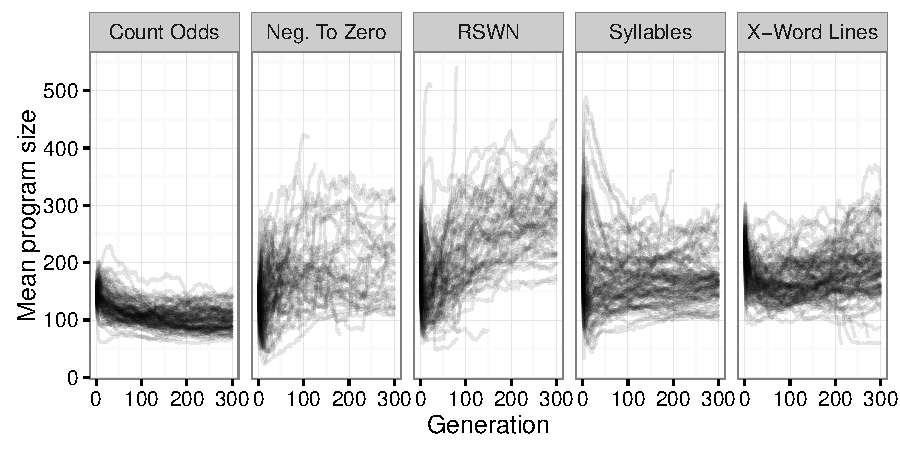
\includegraphics[width=\textwidth]{program_sizes_3x6_relabelled}
\caption{Mean program sizes each generation for 100 runs each of five different software synthesis benchmark problems. ``RSWN'' is an abbreviation for ``Replace Space With Newline''. Note that the max}
\label{fig:programSizes}
\end{figure}

Code bloat without corresponding improvement in fitness has long caused problems in genetic programming \cite{Silva:2009:GPEM, luke:dissertation}. In our experience with uniform genetic operators in Plush, we have not observed code bloat.
Figure~\ref{fig:programSizes}, for example, plots the mean program size of each population over time for each run using the REG genetic operators.
One of the problems (Count Odds) shows a slight \emph{decrease} in average program size, and one (Replace Space With Newline) shows moderate growth. The mean program size for the other three problems remains fairly flat. In these runs, the maximum program size limit for the Count Odds and Negative to Zero problems is 1000, and for the other three problems is 1600. None of the mean program sizes come close to approaching these limits.

Of the uniform genetic operators we describe, only alternation can create a child of a different size than its parent. In fact, alternation has a slight bias toward creating smaller children than their parents, since alternation terminates upon reaching the end of the current parent's genome. This bias may partially account for the bloat control observed here, though children of alternation may also be larger than their parents. On the other hand, even operators that do not change the size of the produced children such as uniform mutation may have anti-bloat effects. For example, a bloated program will likely have more of its instructions replaced by uniform mutation than a smaller program, increasing the chances of functionality-breaking changes.


%While a formal treatment is beyond the scope of this study, we would like to note that our experience with these uniform genetic operators has demonstrated that they avoid many of the unexpected pitfalls of tree-based genetic operators. In particular, we have never observed bloat (or drastic drops in program size) with these uniform operators. Figure~\ref{fig:programSizes}, for example, shows the mean program sizes over time for 100 runs each for five different software synthesis benchmark problems~\cite{Helmuth:2015:GECCO}. One of the problems (Count Odds) shows a slight \emph{decrease} in average program size, and one (Replace Space With Newline) shows a moderate (but not exponential) growth. The mean program sizes for the other three problems remains fairly flat.


\section{Conclusions}

We have described a linear representation (Plush) for structured programs (in the Push programming language), and shown that it allows for uniform genetic operators that produce meaningful structure while solving difficult problems. The central idea of the representation scheme is to use epigenetic markers, attached to instructions and literals, to indicate where structure should be added to programs when they are expressed from the linear genomes. We compared the efficacy of different combinations of uniform genetic operators operating on Plush genomes and showed how the Plush-to-Push translation scheme encourages the expression of programs with structure in appropriate places. We note that the Plush-based system appears to be relatively robust to settings of the genetic operators and that it is capable of solving difficult software synthesis problems without producing significant code bloat.



\begin{acknowledgement}
This material is based upon work supported by the National Science Foundation under Grants No. 1129139 and 1331283. Any opinions, findings, and conclusions or recommendations expressed in this publication are those of the authors and do not necessarily reflect the views of the National Science Foundation.
\end{acknowledgement}

%%%%%%%%%%%%%%%%%%%%%%%% referenc.tex %%%%%%%%%%%%%%%%%%%%%%%%%%%%%%
% sample references
% %
% Use this file as a template for your own input.
%
%%%%%%%%%%%%%%%%%%%%%%%% Springer-Verlag %%%%%%%%%%%%%%%%%%%%%%%%%%
%
% BibTeX users please use
\bibliographystyle{spmpsci}
\bibliography{helmuth}
%

\end{document}
